%!TEX root = ../main.tex

\chapter{Discussione}\label{chp:discussion}
% 
Dopo aver dettagliatamente descritto le caratterstiche dei tre strumenti bioinformatici nel Capitolo\,\ref{chp:CNN-non-coding-variants}, in questo capitolo si paragoneranno i tre tool, sottolineando le proprietà comuni e gli aspetti per cui differiscono in modo da fornire un confornto oggettivo che permette di comprendere in maniera più approfondita le loro performance predittive.

DeepSEA, Basset e DeepSATA, hanno alcune caratterstiche in comune. I tre tool utilizzano lo stesso metodo di codifica della sequenza, il One-Hot encoding, che rende la sequenza luna $M$ in una matrice $M\times 4$, mappando le basi azotate della sequenza in vettori. In questo modo la sequenza può essere processata correttamente dai kernel, che sono delle \acs{PWM} che associano a ciascuna base delle sequenza un peso (o probabilità di occorrenza) in una particolare posizione (Figura\,\ref{fig:PWM}). Infine i tre modelli sono stati allenati attraverso il \acs{SGD} cercando di ottimizzare la stessa funzione obiettivo (cost function): la binary cross entropy (\acs{BCE}).

\vspace{5px}

Nonstante le similarità descritte, i tre strumenti prensentano diverse differenze, soprattutto nella struttura della rete e nel training dataset scelto: la Tabella\,\ref{tab:summary} riassume le caratteristiche principali. \,\hyperref[sec:DeepSEA]{\textsl{DeepSEA}} è composto da tre livelli convoluzionali, ciascuno dei quali viene seguito sempre da un livello \acs{ReLU} e da un livello max-pooling, utilizzato per estrarre le feature dominanti processate dalla convoluzione. I tre livelli convoluzionali contengono rispettivamente 320, 480 e 960 filtri. In seguito è presente un fully-conncted layer che prepara la informazioni per essere valutate nell'output layer, formato da una sigmoide.

Anche \hyperref[sec:Basset]{\textsl{Basset}} è composto da tre livelli convoluzionali ma in aggiunga al \acs{ReLU} layer e al max-pooling layer viene inserito anche un livello di normalizzazione. Sono poi presenti tre livelli fully-connected che sono alternati da altri \acs{ReLU} layer e dei dropout layer, per evitare l'overfitting. Anche in questo caso l'output è calcolato tramite una sigmoide.
% 
\begin{table}[!t]
    \centering
    \caption{Riassunto delle differenza tra i tre tool.}\label{tab:summary}
    \renewcommand{\arraystretch}{2}
    \begin{tabular}{|>{\centering\arraybackslash}m{2cm}|>{\centering\arraybackslash}m{4.5cm}|>{\centering\arraybackslash}m{1.5cm}|>{\centering\arraybackslash}m{1.5cm}|>{\centering\arraybackslash}m{3cm}|} % chktex-file 44
        \hline % chktex-file 44
        \textbf{Modello} & \textbf{Struttura} & \textbf{Kernel} & \textbf{Input} & \textbf{Dataset} \\ 
        \hline\hline % chktex-file 44
        \hyperref[sec:DeepSEA]{\textsl{DeepSEA}} & Tre livelli convoluzionali — ciascuno seguito da un \acs{ReLU} layer e da un max-pooling layer — e un fully-connected layer  &  320, 480, 960 & $1000\times 4$ & \acs{ENCODE}, Roadmap Epigenomics\\ 
        % 
        \hyperref[sec:Basset]{\textsl{Basset}} & Tre livelli convoluzionali — ciascuno seguito da un normalization layer, un \acs{ReLU} layer e da un max-pooling layer — e tre fully-connected layer — alternati da un \acs{ReLU} layer ed un dropout layer &  300, 200, 200 & $600 \times 4$ & \acs{ENCODE}, Roadmap Epigenomics\\ 
        % 
        \hyperref[sec:DeepSATA]{\textsl{DeepSATA}} & Tre livelli convoluzionali — ciascuno seguito da un \acs{ReLU} layer, da un max-pooling layer e da un dropout layer — e un fully-connected layer & 320, 480, 960 & $1000\times 4\times 11$ & \acs{ENCODE}, \acs{NCBI} \acs{SRA}, \acs{GEO}, UC Davis\\ 
        \hline
    \end{tabular}
    \renewcommand{\arraystretch}{1}
\end{table}

Come DeepSEA e Basset, anche \hyperref[sec:DeepSATA]{\textsl{DeepSATA}} è composto da tre livelli di convoluzione, con rispettivamente 320, 480 e 960 kernel. Ad ogni layer convoluzionale segue un \acs{ReLU} layer, un max-pooling layer ed un dropout layer, per prevenire il rischio di overfitting. Ai livelli convoluzionali segue un fully connected layer che processa le informazioni per l'output layer che applica una funzione sigmoide. Si osserva inoltre che in questo modello, a differenza degli altri due, processa un input tridimensionale, volto a fornire più contesto per comprendere in maniera migliore gli eventuali effetti delle mutazioni sulla sequenza.

Gli autori dell'articolo che introduce DeepSATA, dopo aver illustrato il modello e le principali differenza con il suo predecessore DeepSEA, conducono un esperimento dove paragonano le capacità predittive di DeepSEA, Basset e DeepSATA.\@ In particolare, dopo aver allenato i tre modelli sul dataset contenente sequenze di specie animali diverse, tra cui l'uomo, valutano le prestazione dei modelli. Dai risultati del test (Tabella\,\ref{tab:comparison}) si nota che le prestazioni predittive di DeepSATA, anche se non di molto, superano le prestazioni di DeepSEA e di Basset. In particolare si nota una maggiore differenza nelle sequenze genetiche dei maiali, dove il valore \acs{AUC}/\acs{AUROC} è superiore di più di cinque punti percentuale. Nelle altre specie invece, anche se non di tanto, DeepSATA ottiene comunque risultati migliori.
\begin{table}[!h]
    \centering
    \caption{Riassunto del confronto tra DeepSEA, Basset e DeepSATA}\label{tab:comparison}
    \renewcommand{\arraystretch}{2}
    \begin{tabular}{|>{\centering\arraybackslash}p{2cm}|>{\centering\arraybackslash}p{2cm}|>{\centering\arraybackslash}p{2cm}|>{\centering\arraybackslash}p{2cm}|>{\centering\arraybackslash}p{2cm}|>{\centering\arraybackslash}p{2cm}|} % chktex-file 44
        \hline % chktex-file 44
        \textbf{Modello} & \textbf{Topi} & \textbf{Maiali} & \textbf{Bovini} & \textbf{Umani} & \textbf{Polli}\\ 
        \hline\hline % chktex-file 44
        \hyperref[sec:DeepSATA]{\textsl{DeepSATA}} & 0.854 & 0.779 & 0.772 & 0.759 & 0.744 \\ 
        % 
        \hyperref[sec:DeepSEA]{\textsl{DeepSEA}} & 0.796 & 0.775 & 0.769 & 0.755 & 0.736 \\ 
        % 
        \hyperref[sec:Basset]{\textsl{Basset}} & 0.778 & 0.719 & 0.768 & 0.717 & 0.722 \\ 
        \hline
    \end{tabular}
    \renewcommand{\arraystretch}{1}
\end{table}
Dalla Tabella\,\ref{tab:comparison} si nota che i valori \acs{AUROC} di DeepSATA e DeepSEA differiscono di pochi  millesimi tra loro, a differenza dei valori di Basset, che talvolta sono nettamente più bassi rispetto ai valori degli altri due modelli. In particolare sulle sequenze che riguardano il genoma umano si nota una differenza di circa quattro punti percentuale tra Basset e DeepSEA/DeepSATA.\@
% 
\begin{figure}[!b]
    \centering
    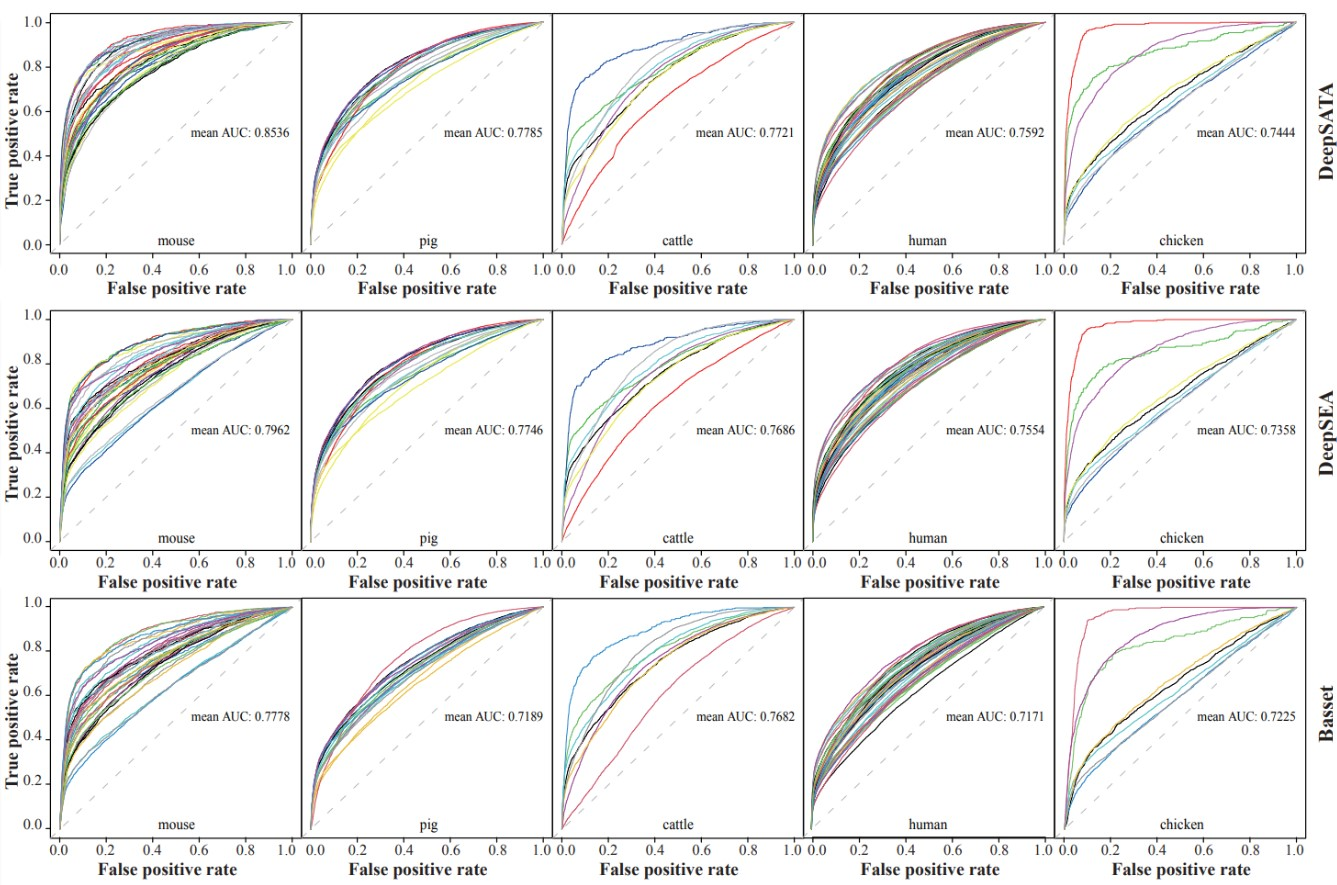
\includegraphics[width=1\textwidth]{assets/imgs/comparison.jpg}
    \caption[Confronto delle prestazioni predittive dei tre tool su diverse specie animali.]{Confronto delle prestazioni predittive dei tre tool su diverse specie animali\,\cite{ma2023deepsata}.}\label{fig:comparison}
\end{figure}
% 
Di conseguenza, la tabella, oltre che ad indicare che DeepSATA abbia capacità predittive migliori rispetto agli altri due strumenti, suggerisce che il modello di DeepSEA riesce a riconoscere in maniera migliore le categorie rispetto a Basset. Le informazioni riportate sulla Tabella\,\ref{tab:comparison} sono anche rappresentate sotto forma di curve \acs{ROC} nella Figura\,\ref{fig:comparison}, dove sono indicate le performance predittive di ciascun modello a seconda delle specie animali in esame.

\begin{comment}
    In our study, we utilized DeepSATA to evaluate its predictive capabilities for chromatin features in five distinct species: mice, pigs, cattle, humans, and chickens. We collected open chromatin accessibility datasets and corresponding transcription factor binding motifs, which are summarized in Table 1 and Supplementary Tables S1 and S2. The performance of the DeepSATA, DeepSEA, and Basset models was assessed for each species by comparing their average AUC values across different chromatin features. DeepSATA demonstrated superior performance across all species, with average AUC values of 0.854, 0.779, 0.772, 0.759, and 0.744 for mice, pigs, cattle, humans, and chickens, respectively (Figure 2A and Supplementary Table S3). In comparison, DeepSEA had average AUC values of 0.796, 0.775, 0.769, 0.755, and 0.736, respectively (Figure 2B and Supplementary Table S3), while Basset had average AUC values of 0.778, 0.719, 0.768, 0.717, and 0.722, respectively (Figure 2C and Supplementary Table S3). It is worth noting that DeepSATA consistently outperformed DeepSEA and Basset in all chromatin features for pigs and mice (Supplementary Table S3). The relative improvement was particularly significant in the cerebrum tissue of the mice, where DeepSATA achieved an AUC of 0.829 compared to DeepSEA’s 0.659 for female mice and an AUC of 0.828 compared to DeepSEA’s 0.653 for male mice, representing a relative improvement of over 25%. Interestingly, our findings indicate that the DeepSATA, DeepSEA, and Basset models performed better for the Duroc pig breed compared to other pig breeds (Supplementary Table S3). This suggests a superior ability to recognize regulatory functional patterns in the non-coding genomic regions  pecific to Duroc pigs. In the case of cattle, the chromatin feature of the hypothalamus was most effectively captured, with AUC values of 0.887 for DeepSATA, 0.883 for DeepSEA, and 0.895 for Basset (Supplementary Table S3). What particularly encouraged us was the remarkable performance of DeepSATA in accurately recognizing the regulatory patterns of the cerebellum in chickens, achieving AUC values as high as 0.972, while DeepSEA achieved 0.971 and Basset achieved 0.953 (Supplementary Table S3). Additionally, in the following analysis, we selected DeepSEA as the baseline comparison, since it achieved better prediction performance compared with Basset. Overall, these results clearly demonstrate the effectiveness of DeepSATA in accurately identifying the regulatory patterns of chromatin features in different animal species
\end{comment}
